\documentclass[11pt, letterpaper]{cmu}

\usepackage[all]{hypcap}
\usepackage[comma,numbers,sort,compress]{natbib}
\usepackage{hyperref}[citecolor=magenta]

\hypersetup{
    colorlinks = true,
    citecolor = {magenta},
}

\usepackage{microtype}
\usepackage{graphicx}
\usepackage{subfigure}
\usepackage{booktabs}
\usepackage{float}

\usepackage{amsmath}
\usepackage{amssymb}
\usepackage{mathtools}
\usepackage{amsthm}
\usepackage{mathrsfs}
\usepackage{nicefrac}
\usepackage{dsfont}
\usepackage{enumitem}
% \usepackage{minted}
\usepackage{float}

\setlength\parindent{0pt}
% \setminted[python]{frame=lines, breaklines, framesep=2mm, fontsize=\footnotesize, numbersep=5pt}

\usepackage{xspace}
\usepackage[capitalize,noabbrev]{cleveref}
\bibliographystyle{plainnat}
\usepackage{subcaption}
\usepackage{wrapfig}
\usepackage{lipsum}
\usepackage{listings}

\usepackage{amsmath}
\usepackage{amssymb}
\usepackage{mathtools}
\usepackage{amsthm}
\usepackage{bbm}
\usepackage{fleqn, tabularx}
\usepackage{multirow}
\usepackage[export]{adjustbox}
\usepackage{colortbl}

\usepackage{algpseudocode}
\usepackage{setspace}

\usepackage{color}
\definecolor{deepblue}{rgb}{0,0,0.5}
\definecolor{deepred}{rgb}{0.6,0,0}
\definecolor{deepgreen}{rgb}{0,0.5,0}
\definecolor{boost_correct_to_correct}{HTML}{66C2A5}
\definecolor{default_correct_to_correct}{HTML}{fc8d62}
\definecolor{dup_correct_to_correct}{HTML}{8da0cb}
\definecolor{new_correct_to_correct}{HTML}{e78ac3}

\newcommand\pythonstyle{\lstset{
basicstyle=\ttfamily\footnotesize,
language=Python,
morekeywords={self, clip, exp, mse_loss, uniform_sample, concatenate, logsumexp},
keywordstyle=\color{deepblue},
emph={MyClass,__init__},
emphstyle=\color{deepred},
stringstyle=\color{deepgreen},
frame=single,
showstringspaces=false
}}


\lstnewenvironment{python}[1][]
{
\pythonstyle
\lstset{#1}
}
{}


\newcommand\pythonexternal[2][]{{
\pythonstyle
\lstinputlisting[#1]{#2}}}

\newcommand\pythoninline[1]{{\pythonstyle\lstinline!#1!}}


%% editing comment
\newcommand{\cmt}[1]{{\footnotesize\textcolor{red}{#1}}}
\newcommand{\cmto}[1]{{\footnotesize\textcolor{orange}{#1}}}
\newcommand{\note}[1]{\cmt{Note: #1}}
% \newcommand{\todo}[1]{\cmt{TO-DO: #1}}
\newcommand{\question}[1]{\cmto{Question: #1}}
\newcommand{\ak}[1]{{\textcolor{red}{#1}}}
\newcommand{\aviral}[1]{{\textcolor{red}{#1}}}
\newcommand{\edits}[1]{\textcolor{blue}{#1}}
\newcommand{\editsred}[1]{\textcolor{red}{#1}}
\newcommand{\editsp}[1]{\textcolor{purple}{#1}}
\newcommand{\editsv}[1]{\textcolor{magenta}{#1}}

% \newcommand{\edits}[1]{\textcolor{black}{#1}}
% \newcommand{\editsred}[1]{\textcolor{black}{#1}}
% \newcommand{\editsp}[1]{\textcolor{black}{#1}}
% \newcommand{\editsv}[1]{\textcolor{black}{#1}}


%% abbreviations
\newcommand{\x}{\mathbf{x}}
\newcommand{\z}{\mathbf{z}}
\newcommand{\y}{\mathbf{y}}
\newcommand{\w}{\mathbf{w}}
\newcommand{\data}{\mathcal{D}}
\newcommand{\E}{\mathbb{E}}

\newcommand{\etal}{{et~al.}\ }
\newcommand{\eg}{\emph{e.g.},\ }
\newcommand{\ie}{\emph{i.e.},\ }
\newcommand{\nth}{\text{th}}
\newcommand{\pr}{^\prime}
\newcommand{\tr}{^\mathrm{T}}
\newcommand{\inv}{^{-1}}
\newcommand{\pinv}{^{\dagger}}
\newcommand{\real}{\mathbb{R}}
\newcommand{\gauss}{\mathcal{N}}
% \newcommand{\norm}[1]{\left|#1\right|}
% \newcommand{\trace}{\text{tr}}

%% specifics for the paper
\newcommand{\reward}{r}
\newcommand{\policy}{\pi}
\newcommand{\mdp}{\mathcal{M}}
\newcommand{\states}{\mathcal{S}}
\newcommand{\actions}{\mathcal{A}}
\newcommand{\observations}{\mathcal{O}}
\newcommand{\transitions}{T}
\newcommand{\initstate}{d_0}
\newcommand{\freq}{d}
\newcommand{\obsfunc}{E}
\newcommand{\initial}{\mathcal{I}}
\newcommand{\horizon}{H}
\newcommand{\rewardevent}{R}
\newcommand{\probr}{p_\rewardevent}
\newcommand{\metareward}{\bar{\reward}}
\newcommand{\discount}{\gamma}
\newcommand{\behavior}{{\pi_\beta}}
\newcommand{\bellman}{\mathcal{B}}
\newcommand{\qparams}{\phi}
\newcommand{\qparamset}{\Phi}
\newcommand{\qset}{\mathcal{Q}}
\newcommand{\batch}{B}
\newcommand{\qfeat}{\mathbf{f}}
\newcommand{\Qfeat}{\mathbf{F}}
\newcommand{\hatbehavior}{\hat{\pi}_\beta}

\newcommand{\traj}{\tau}

\newcommand{\pihi}{\pi^{\text{hi}}}
\newcommand{\pilo}{\pi^{\text{lo}}}
\newcommand{\ah}{\mathbf{w}}

% \newcommand{\proj}{\Pi}

\newcommand{\loss}{\mathcal{L}}
\newcommand{\eye}{\mathbf{I}}

\newcommand{\model}{\hat{p}}

\newcommand{\pimix}{\pi_{\text{mix}}}

\newcommand{\pib}{\bar{\pi}}
\newcommand{\epspi}{\epsilon_{\pi}}
\newcommand{\epsmodel}{\epsilon_{m}}

\newcommand{\return}{\mathcal{R}}

%% math
\newcommand{\cY}{\mathcal{Y}}
\newcommand{\cX}{\mathcal{X}}
\newcommand{\en}{\mathcal{E}}
\newcommand{\bu}{\mathbf{u}}
\newcommand{\bv}{\mathbf{v}}
% \newcommand{\bb}{\mathbf{b}}
\newcommand{\bd}{\mathbf{d}}
\newcommand{\be}{\mathbf{e}}
\newcommand{\by}{\mathbf{y}}
\newcommand{\bx}{\mathbf{x}}
\newcommand{\bz}{\mathbf{z}}
\newcommand{\bw}{\mathbf{w}}
\newcommand{\boldm}{\mathbf{m}}
\newcommand{\bo}{\mathbf{o}}
% \newcommand{\bs}{\mathbf{s}}
% \newcommand{\ba}{\mathbf{a}}
\newcommand{\bs}{\mathbf{s}}
\newcommand{\ba}{\mathbf{a}}
\newcommand{\bM}{\mathbf{M}}
\newcommand{\ot}{\bo_t}
% \newcommand{\st}{\bs_t}
\newcommand{\at}{\ba_t}
\newcommand{\op}{\mathcal{O}}
\newcommand{\opt}{\op_t}
\newcommand{\kl}{D_\text{KL}}
\newcommand{\tv}{D_\text{TV}}
\newcommand{\ent}{\mathcal{H}}
\newcommand{\bG}{\mathbf{G}}
\newcommand{\byk}{\mathbf{y_k}}
\newcommand{\bI}{\mathbf{I}}
\newcommand{\bg}{\mathbf{g}}
\newcommand{\bV}{\mathbf{V}}
\newcommand{\bD}{\mathbf{D}}
\newcommand{\bR}{\mathbf{R}}
\newcommand{\bQ}{\mathbf{Q}}
\newcommand{\bA}{\mathbf{A}}
\newcommand{\bN}{\mathbf{N}}
\newcommand{\bS}{\mathbf{S}}
\newcommand{\bW}{\mathbf{W}}
\newcommand{\bU}{\mathbf{U}}
\newcommand{\bO}{\mathbf{O}}
\newcommand{\leftnorm}{\left\vert \left\vert}
\newcommand{\rightnorm}{\right\vert \right\vert}

\newcommand{\bzhi}{\bz^\text{hi}}
\newcommand{\expected}{\mathbb{E}}
% \newcommand{\srank}{\text{srank}}
% \newcommand{\rank}{\text{rank}}
\newcommand{\deepnet}{\bW_N(k, t) \bW_\phi(k, t)}
\newcommand{\features}{\bW_\phi(k, t)}
\newcommand{\stateactioni}{[\bs_i; \ba_i]}
% \newcommand{\diag}{\text{\textbf{diag}}}
\newcommand{\cosine}{\text{cos}}


\def\thetaP{\theta^{\prime}}
\def\cf{\emph{c.f.}\ }
\def\vs{\emph{vs}.\ }
\def\etc{\emph{etc.}\ }
\def\Eqref#1{Equation~\ref{#1}}
\def\ss#1{\scriptsize #1}

\newenvironment{repeatedthm}[1]{\@begintheorem{#1}{\unskip}}{\@endtheorem}

% \DeclareMathOperator\supp{supp}
\newcommand{\methodname}{Cal-QL}
\newcommand{\aliasingproblemname}{bootstrapping aliasing}
\newcommand{\Aliasingproblemname}{Bootstrapping aliasing}
\newcommand{\AliasingProblemName}{Bootstrapping Aliasing}
\newcommand{\simnorm}{\mathrm{sim}_{\mathrm{n}}^\pi}
\newcommand{\simunnorm}{\mathrm{sim}_{\mathrm{u}}^\pi}

% colors from moderncv that are especially appealing
\definecolor{blanchedalmond}{rgb}{1.0, 0.92, 0.8}
\definecolor{carmine}{rgb}{0.59, 0.0, 0.09}
\definecolor{lightblue}{rgb}{0.22,0.45,0.70}% light blue


\newcommand{\gjt}[1]{\textcolor{red}{[gjt: #1]}}
% \newcommand{\rebuttal}[1]{\textcolor{red}{#1}}
\newcommand{\rebuttal}[1]{#1}
\newcommand{\scenario}[1]{\textcolor{lightblue}{S#1}}
\newcommand{\technique}[1]{\textcolor{carmine}{T#1}}
\newcommand{\application}[1]{\textcolor{carmine}{A#1}}

\def\bellmanop{T^\circ}
\def\qop{Q^\circ}
\def\qpi{Q^\pi}
\def\qs{Q^*}
\def\Qstar{Q^*}
\def\Qt{Q_{\theta}}
\def\Qtp{Q_{\thetaP}}
\def\ld{\ell_{\lambda}}


%%% SZ.1.11: added my math defs below:

\newtheorem{theorem}{Theorem}[section]
\newtheorem{sketchtheorem}{Sketch Theorem}[section]
\newtheorem{lemma}[theorem]{Lemma}
\newtheorem{corollary}[theorem]{Corollary}
\newtheorem{proposition}[theorem]{Proposition}
\newtheorem{definition}[theorem]{Definition}
\newtheorem{conjecture}[theorem]{Conjecture}
\newtheorem{problem}[theorem]{Problem}
\newtheorem{formulation}[theorem]{Formulation}
\newtheorem{claim}[theorem]{Claim}
\newtheorem{remark}[theorem]{Remark}
\newtheorem{example}[theorem]{Example}
\newtheorem{assumption}[theorem]{Assumption}
\newtheorem{exercise}[theorem]{Exercise}


\newcommand{\indep}{\rotatebox[origin=c]{90}{$\models$}}

\renewcommand{\mathbf}{\boldsymbol}

\newcommand{\conv}{\circledast}
\newcommand{\mb}{\mathbf}
\newcommand{\mc}{\mathcal}
\newcommand{\mf}{\mathfrak}
\newcommand{\md}{\mathds}
\newcommand{\bb}{\mathbb}
\newcommand{\msf}{\mathsf}
\newcommand{\mcr}{\mathscr}
\newcommand{\magnitude}[1]{ \left| #1 \right| }
\newcommand{\set}[1]{\left\{ #1 \right\}}
\newcommand{\condset}[2]{ \left\{ #1 \;\middle|\; #2 \right\} }


\newcommand{\reals}{\bb R}
\newcommand{\proj}{\mathrm{proj}}

\newcommand{\eps}{\varepsilon}
\newcommand{\R}{\reals}
\newcommand{\Cp}{\bb C}
\newcommand{\Z}{\bb Z}
\newcommand{\N}{\bb N}
\newcommand{\Sp}{\bb S}
\newcommand{\Ba}{\bb B}
\newcommand{\indicator}[1]{\mathbbm 1\left\{#1\right\}}
\renewcommand{\P}{\mathbb{P}}
\newcommand{\rvline}{\hspace*{-\arraycolsep}\vline\hspace*{-\arraycolsep}}
\makeatletter
\def\Ddots{\mathinner{\mkern1mu\raise\p@
\vbox{\kern7\p@\hbox{.}}\mkern2mu
\raise4\p@\hbox{.}\mkern2mu\raise7\p@\hbox{.}\mkern1mu}}
\makeatother
% to declare new operator
% \DeclareMathOperator{\xxx}{xxx}

%% Other definitions

\newcommand{\event}{\mc E}

\newcommand{\e}{\mathrm{e}}
\newcommand{\im}{\mathrm{i}}
\newcommand{\rconcave}{r_\fgecap}
\newcommand{\Lconcave}{\mc L^\fgecap}
\newcommand{\rconvex}{r_\fgecup}
\newcommand{\Rconvex}{R_\fgecup}
\newcommand{\Lconvex}{\mc L^\fgecup}

\newcommand{\wh}{\widehat}
\newcommand{\wt}{\widetilde}
\newcommand{\ol}{\overline}


\newcommand{\betaconcave}{\beta_\fgecap}
\newcommand{\betagrad}{\beta_{\mathrm{grad}}}

\newcommand{\norm}[2]{\left\| #1 \right\|_{#2}}
\newcommand{\abs}[1]{\left| #1 \right|}
\newcommand{\row}[1]{\text{row}\left( #1 \right)}
\newcommand{\innerprod}[2]{\left\langle #1,  #2 \right\rangle}
\newcommand{\prob}[1]{\bb P\left[ #1 \right]}
\newcommand{\expect}[1]{\bb E\left[ #1 \right]}
\newcommand{\function}[2]{#1 \left(#2\right}
\newcommand{\integral}[4]{\int_{#1}^{#2}\; #3\; #4}
\newcommand{\paren}[1]{\left( #1 \right)}
\newcommand{\brac}[1]{\left[ #1 \right]}
\newcommand{\Brac}[1]{\left\{ #1 \right\}}

% Adding new defs here
\newcommand{\moff}{m_\mr{off}}
\newcommand{\mon}{m_\mr{on}}
\newcommand{\EmpiricalOffline}{\wh{\bb E}_{\mc D^\nu_h}}
\newcommand{\EmpiricalOnline}{\wh{\bb E}_{\mc D^\tau_h}}
\newcommand{\Deltaoff}{\Delta_\mr{off}}
\newcommand{\Deltaon}{\Delta_\mr{on}}
\newcommand{\Vmax}{V_{\max}}
\newcommand{\regret}{\mr{Reg}}
\newcommand{\regreton}{\mr{Sub}_{\mr {on}}}
\newcommand{\regretoff}{\mr{Sub}_{\mr {off}}}
\newcommand{\Doff}{\mc D_\mr{off}}
\newcommand{\Don}{\mc D_\mr{on}}
\newcommand{\piref}{\pi_\mr{ref}}

\newcommand{\nt}[1]{{\color{purple}{\bf [Next: #1]}}}
\newcommand{\here}{{\color{purple}{\bf [Writing here]}}}
% \newcommand{\todo}{{\color{purple}{\bf [TODO]}}}
\newcommand{\sz}[1]{{\color{blue}{\bf [Simon: #1]}}}
% \newcommand{\note}[1]{{\color{red}{\bf [note: #1]}}}
\newcommand{\mr}{\mathrm}
\newcommand{\sym}{\mathrm{Sym}}
\newcommand{\sks}{\mathrm{Skew}}
\newcommand{\inprod}[2]{\langle#1,#2\rangle}
\newcommand{\parans}[1]{\left(#1\right}
\newcommand{\clip}{\msf{clipped}}
\newcommand{\beha}{\msf b}
\numberwithin{equation}{section}

\definecolor{amaranth}{rgb}{0.9, 0.17, 0.31}
\definecolor{antiquebrass}{rgb}{0.8, 0.58, 0.46}
\definecolor{antiquefuchsia}{rgb}{0.57, 0.36, 0.51}
% \definecolor{chromeyellow}{rgb}{1.0, 0.65, 0.0}
% \definecolor{chromeyellow}{rgb}{0.82, 0.41, 0.12}
% \definecolor{chromeyellow}{rgb}{1.0, 0.5, 0.31}
\definecolor{chromeyellow}{rgb}{0.31, 0.47, 0.26}


\def \endprf{\hfill {\vrule height6pt width6pt depth0pt}\medskip}
% \newenvironment{proof}{\noindent {\bf Proof} }{\endprf\par}

% \newcommand{\qed}{{\unskip\nobreak\hfil\penalty50\hskip2em\vadjust{}
%            \nobreak\hfil$\Box$\parfillskip=0pt\finalhyphendemerits=0\par}}

%% table color
\usepackage[dvipsnames]{xcolor}
% \definecolor{maj5}{HTML}{009ADE}
% \definecolor{maj5Imp}{HTML}{0D4A70}
\definecolor{maj5}{HTML}{2b8cbe}
\definecolor{maj5Imp}{HTML}{084081}

\definecolor{seq5wo}{HTML}{d95f0e}
\definecolor{seq5woImp}{HTML}{662506}

\definecolor{seq5w}{HTML}{6a51a3}
\definecolor{seq5wImp}{HTML}{3f007d}

\definecolor{selfwo}{HTML}{d95f0e}
\definecolor{selfwoImp}{HTML}{662506}

\definecolor{selfw}{HTML}{6a51a3}
\definecolor{selfwImp}{HTML}{3f007d}

\definecolor{glorewo}{HTML}{d95f0e}
\definecolor{glorewoImp}{HTML}{662506}

\definecolor{glorew}{HTML}{6a51a3}
\definecolor{glorewImp}{HTML}{3f007d}

% \definecolor{selfw}{HTML}{00718B}
% \definecolor{selfwImp}{HTML}{003147}

% \definecolor{selfwo}{HTML}{E32977}
% \definecolor{selfwoImp}{HTML}{8F003B}

% \definecolor{glorew}{HTML}{00718B}
% \definecolor{glorewImp}{HTML}{003147}

% \definecolor{glorewo}{HTML}{E32977}
% \definecolor{glorewoImp}{HTML}{8F003B}

\definecolor{vstar}{HTML}{d95f0e}
\definecolor{vstarImp}{HTML}{662506}








\makeatletter
\def\mathcolor#1#{\@mathcolor{#1}}
\def\@mathcolor#1#2#3{%
  \protect\leavevmode
  \begingroup
    \color#1{#2}#3%
  \endgroup
}
\makeatother

\usepackage[textsize=tiny]{todonotes}
\usepackage{algorithm}
\usepackage{amssymb}


\usepackage[skins,theorems]{tcolorbox}
\Crefformat{equation}{#2Eq.\;(#1)#3}

\Crefformat{figure}{#2Figure #1#3}
\Crefformat{assumption}{#2Assumption #1#3}
\Crefname{assumption}{Assumption}{Assumptions}

\usepackage{crossreftools}
\pdfstringdefDisableCommands{
    \let\Cref\crtCref
    \let\cref\crtcref
}
\newcommand{\creftitle}[1]{\crtcref{#1}}

\usepackage[suppress]{color-edits}

\newcommand\numberthis{\addtocounter{equation}{1}\tag{\theequation}}

\usepackage{dsfont}
\usepackage{nicefrac}

\newtcolorbox{analysisbox}[1][]{
    enhanced jigsaw,
    colback=white,
    colframe=blue!75!black,
    fonttitle=\bfseries,
    boxsep=5pt,
    left=5pt,
    right=5pt,
    top=5pt,
    bottom=5pt,
    title=#1,
}
\newcommand{\mistake}[1]{\sethlcolor{highlightmistake}\hl{#1}\sethlcolor{yellow}}
\newcommand{\correct}[1]{\sethlcolor{highlightcorrect}\hl{#1}\sethlcolor{yellow}}
\newcommand{\cmark}{\ding{51}}
\newcommand{\xmark}{\ding{55}}

\tcbset{
  aibox/.style={
    width=\linewidth,
    top=8pt,
    bottom=4pt,
    colback=blue!6!white,
    colframe=black,
    colbacktitle=black,
    enhanced,
    center,
    attach boxed title to top left={yshift=-0.1in,xshift=0.15in},
    boxed title style={boxrule=0pt,colframe=white,},
  }
}
\newtcolorbox{AIbox}[2][]{aibox,title=#2,#1}
\definecolor{lightblue}{rgb}{0.22,0.45,0.70}% light blue

\usepackage{pifont}
\usepackage{soul}
\definecolor{highlightmistake}{RGB}{255, 179, 179}
\definecolor{highlightcorrect}{RGB}{179, 255, 179}
\newcommand{\rr}[1]{\textbf{\color{green}[RR: #1]}}

\title{Post-training is only as good as its reward:\\ an RL acquisition problem inside genetic perturbation design}

% \reportnumber{}

\author[1]{Yixi Zhao}
\author[1]{Zhangchi (Allen) Chen}

\affil[1]{Carnegie Mellon University}

\correspondingauthor{yixiz@andrew.cmu.edu}

\hyphenation{pre-print}

\begin{abstract}
Our proposal was to post-train an inverse-design generator of genetic perturbations with
RL, using a forward oracle (GEARS) for cycle-consistency and biological rewards. Three
weeks of measurement changed the formulation. We first show that on this task the
\emph{reward oracle}, not the generator, is the binding constraint: a parameter-free
nearest-centroid match identifies the correct perturbation $86.6\%$ of the time, while
ranking the same candidates by GEARS reaches $8.3\%$ --- a 78-point gap that no amount of
generator post-training can close, because the reward cannot see the headroom. We then
re-scope to a genuinely RL-shaped problem on the same scientific task: a budgeted
\emph{acquisition MDP} --- which $100$ of $437$ candidate genes to measure so that a
cheap predictor built from the measurements best identifies the rest. We implement three
RL methods --- REINFORCE over a Plackett--Luce policy, a learned critic used as a control
variate, and a PPO feature policy with GRPO-style group-relative advantages --- and,
given the information greedy uses, all three beat greedy ($1.35$--$1.59\times$ random vs
greedy's $1.24\times$, winning $85$ of $90$ paired runs). The gain is explained,
mechanistically, by a reward whose one-step signal correlates only $r{=}0.17$ with the
quantity that matters, which a feature critic predicts at $r{=}0.26$. We also report a
clean \emph{negative} result: in the prospective (blind) regime, five learned policies tie
a 1970s facility-location heuristic, and the scale hypothesis we had for it is refuted
rather than merely unconfirmed. Published methods on the identical task (IterPert, eight
active-learning baselines, three data-valuation methods) leave both conclusions standing.
\end{abstract}

\begin{document}

\maketitle

\section{Project Overview and Motivation}

\textbf{Original goal.} Inverse design of genetic perturbations: given a desired target
cell state, propose the perturbation(s) that produce it. Our proposal was to take a
pretrained inverse-design generator and \emph{post-train it with RL}, using a forward
oracle (GEARS~\citep{roohani2024gears}) to supply a cycle-consistency term and rewards for
properties supervised models ignore --- selectivity, sparsity, pathway avoidance. The
motivation is real: wet-lab perturbation screens are expensive, and a model that proposes
\emph{which} experiment to run, optimised for arbitrary non-differentiable criteria, is
exactly the kind of black-box-reward problem RL is for~\citep{olivecrona2017reinvent}.

\textbf{What changed, and why.} Before building the RL loop we measured the two things it
depends on: the reward oracle, and the headroom the oracle leaves. Both came back negative
for the original plan and positive for a sharper one.
\begin{enumerate}[leftmargin=1.4em,itemsep=1pt,topsep=2pt]
  \item \textbf{The reward oracle is the bottleneck, not the generator}
  (\Cref{sec:oracle}). Any oracle-driven method --- a supervised inverse map, guidance of a
  frozen prior, or an RL policy rewarded by the oracle --- is capped by the oracle's
  discrimination, and that cap sits far below a trivial lookup baseline. Post-training a
  \emph{generator} cannot recover headroom the \emph{reward} cannot see.
  \item \textbf{The genuinely RL-shaped sub-problem is acquisition, not generation}
  (\Cref{sec:mdp}). The atlas of measured perturbations is itself a choice. Deciding
  which perturbations to measure, under a budget, so that a downstream predictor
  generalises to the rest, is a combinatorial MDP with a discrete action space and a
  non-differentiable, high-variance reward --- the regime in which variance reduction,
  learned baselines and policy generalisation are the tools, not an afterthought.
\end{enumerate}
We therefore keep the scientific target (identify perturbations from a cell state) and the
RL commitment, but move the policy from ``generate a perturbation'' to ``choose the next
measurement.'' This is the same reframing REINVENT-style design and active experimental
design share; it makes the RL contribution measurable against honest baselines rather than
asserted. The rest of this report is the evidence for the move and the RL results it
enables.

\section{Progress and Technical Work So Far [13 points]}

\subsection{The reward oracle is the binding constraint}
\label{sec:oracle}

We built one identical task --- given a target state (pseudo-bulk of pooled held-out
cells), rank the candidate perturbations --- and scored it with three rungs so they
subtract. The \emph{ceiling} ranks by the $\Delta$-signature \emph{measured} from a disjoint
half of the cells (not a usable designer, but a bound on what any method could extract from
the target). The \emph{oracle} rung ranks by the signature GEARS \emph{predicts}; every
oracle-driven method is capped here. On Norman~\citep{norman2019gi}, with a 128-cell target,
the ceiling is $86.6\%$ top-1 and the GEARS rung is $8.3\%$ --- a \textbf{78-point gap},
measured with the official checkpoint on data it was trained on (Table~\ref{tab:ladder}).
Pooling more cells raises the ceiling and leaves the oracle flat near $10\%$, so the limit
is the oracle's prediction error, not noise in the target. On fidelity GEARS does not even
beat a predictor that ignores \emph{which} perturbation was applied: median cosine to the
measured effect is $0.691$ for GEARS vs $0.696$ for the average effect, and GEARS wins on
only $44.8\%$ of conditions.

\begin{table}[h]
\centering\small
\begin{tabular}{rrrrr}
\toprule
Cells pooled & Ceiling & GEARS oracle & Gap (pts) & Median rank (ceil $\to$ oracle)\\
\midrule
1   & 25.4\% & 4.2\% & 21.2 & 6 $\to$ 36\\
32  & 73.9\% & 11.4\% & 62.5 & 1 $\to$ 12\\
\textbf{128} & \textbf{86.6\%} & \textbf{8.3\%} & \textbf{78.3} & \textbf{1 $\to$ 13}\\
\bottomrule
\end{tabular}
\caption{The inverse-design ladder on Norman (rank 230 candidates). The ceiling climbs with
more cells; the oracle does not. Any method rewarded by GEARS lives on the oracle rung.}
\label{tab:ladder}
\end{table}

\textbf{Where any headroom actually lives (\Cref{fig:headroom}).} A perturbation the atlas
has already measured needs no model --- inverse design is then a lookup. Headroom can only
exist for a candidate with \emph{no} atlas entry, and there are exactly three ways that
happens, worth very different amounts. \emph{Unseen pairs} are not a gap: adding two
single-gene signatures reaches $71.6\%$ against a $71.1\%$ ceiling (100\% of the headroom),
while GEARS, \emph{trained on those combinations}, gets $16.1\%$ --- four times worse than
arithmetic. \emph{Unseen contexts} (a gene in another cell line) are half irreducible: the
disattenuated cross-context cosine has median $0.42$, i.e.\ the same gene genuinely acts
differently elsewhere. Only the \emph{unseen gene} axis is a real gap --- high ceiling
($32$--$89\%$), every cheap predictor (GO-similarity kNN, co-response kNN, the published
linear baseline~\citep{ahlmanneltze2025linear}) stuck at $0.8$--$1.9\%$ top-1. The failure
is \emph{discrimination}, not fidelity: GO-kNN reaches $\sim\!70\%$ of the noise-ceiling
cosine but predicts roughly the same direction for every gene.

\begin{figure}[h]
\centering
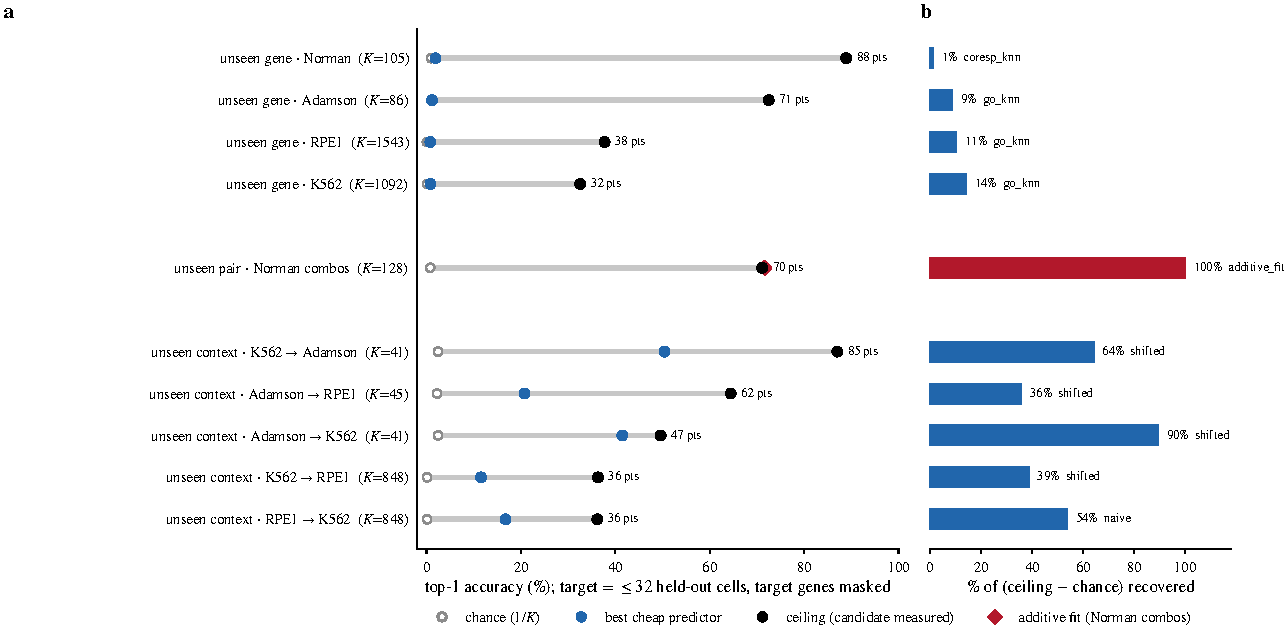
\includegraphics[width=\linewidth]{figures/fig13_headroom_by_axis.pdf}
\caption{\textbf{Of three ways a candidate can be ``unseen,'' only one has headroom.}
\textbf{a}, for each axis/dataset, chance (1/$K$, open), the best cheap predictor (blue;
red diamond = additive fit on Norman combos) and the measured ceiling (black); the label is
the ceiling$-$chance gap. \textbf{b}, the fraction of that gap the cheap predictor recovers
(MRR). Target = $\le$32 held-out cells, with every candidate's own target gene masked (a
design target carries no knocked-down-gene fingerprint). Unseen pairs are arithmetic (100\%
recovered); unseen context is partly irreducible; the four \emph{unseen-gene} rows are the
only place a method has somewhere to go.}
\label{fig:headroom}
\end{figure}

This is a reframing, not a failure: it says a generator trained by distribution matching
has no measurable headroom to beat here, and it isolates the one open prediction problem
(predict an unseen gene's effect specifically enough to tell it from $\sim$1{,}000 others).
It also tells us the RL leverage is \emph{not} in re-scoring a fixed oracle's output: we
verified that a rank reward applied to the same GO-kNN predictions (centre + whiten,
information-preserving) does \emph{not} recover discrimination, which also rules out
contrastive learning for the same reason --- the limit is the input representation, not the
loss.

\subsection{The acquisition MDP}
\label{sec:mdp}

Someone chose the $\sim$1{,}092 genes in the K562 screen~\citep{replogle2022perturbseq}.
Treat that choice as the policy. We define an offline MDP, simulated against \emph{real}
measurements (no learned oracle in the loop, so every episode is a batch of matrix
operations):
\[
\text{state } s_t = \text{genes measured so far};\quad
\text{action } a_t \in \mathcal{A}\setminus s_t;\quad
\text{transition: reveal } a_t\text{'s true signature};\quad
r = \text{retrieval MRR on held-out genes.}
\]
The budget is $B{=}100$ of $|\mathcal{A}|{=}437$ candidate genes, spent in $4$ rounds of
$25$; after each round a GO-kNN predictor is refit from the chosen genes and scored, by mean
reciprocal rank, on a disjoint \emph{report} set the policy never sees. We split genes three
ways --- \texttt{act} (choosable), \texttt{rew} (the reward's genes), \texttt{rep} (report,
only a cheating bound ever sees it) --- so a policy is always rewarded on genes its features
could not observe. Two information regimes frame the whole study:
\begin{description}[leftmargin=1.2em,itemsep=1pt,topsep=2pt]
  \item[Peek.] every non-report signature is visible, including a candidate's before it is
  chosen. This is exactly greedy's information (greedy scores a candidate by inserting its
  real signature), so peek is the \emph{fair} comparison to greedy. It is atlas
  compression: which measured genes best predict the rest.
  \item[Blind.] a signature is revealed only once measured; the policy trains only on the
  already-measured atlas. This is genuine prospective experimental design.
\end{description}
Two diagnostics establish the problem is RL-shaped rather than a search nuisance. First,
the reward is \emph{high-variance, not merely hard}: greedy drives its own objective to
$0.72$ on $25$ reward genes yet delivers $0.168$ held out --- \emph{worse than random} ---
and the harm vanishes monotonically as the reward estimate improves (greedy with $400$
reward genes reaches $+24\%$). Second, the prize is large: an oracle that cheats by
selecting on the report genes reaches $2.0$--$2.2\times$ random, so greedy's $\sim\!1.2\times$
leaves most of it on the table. The lever is reward variance --- precisely what learned
baselines and policy generalisation address.

\subsection{Three RL methods, each testing a different reason greedy falls short}
\label{sec:methods}

All three optimise $J(\pi)=\mathbb{E}_{S\sim\pi}[R(S)]$ over size-$B$ gene sets $S$, differing
in what is learned and therefore in which explanation of greedy's shortfall they probe.

\textbf{(1) REINFORCE~\citep{williams1992reinforce} over a Plackett--Luce policy (search).} One logit $\theta_g$ per
candidate; a set is drawn by sampling $B$ genes without replacement
(Plackett--Luce~\citep{plackett1975luce}), giving
$\nabla_\theta J = \mathbb{E}\big[(R(S)-b)\,\nabla_\theta \log \pi_\theta(S)\big]$ with a
leave-one-out baseline $b$ across the episode's samples for variance reduction. This changes
only the optimiser, not greedy's information or objective. A \texttt{resampled} variant
draws fresh reward genes each episode. REINFORCE reaches a \emph{higher value of greedy's
own reward} (aux MRR $0.233$ vs $0.193$ on K562): with $470$--$850$ reward genes greedy is
not mainly overfitting, it is a poor optimiser of a non-submodular set objective (adding a
gene can evict a better neighbour from a target's top-10).

\textbf{(2) Learned critic as a control variate (reward estimate).} We fit a one-step value
$\hat V_\phi(g)$ --- the \emph{held-out} gain of measuring gene $g$ --- from features alone
($\gamma{=}0$), never seeing the held-out genes. Used greedily it is a cheap policy; used as
a control variate it shrinks greedy's empirical gain toward it,
$\tilde g(g)=\lambda\,\hat V_\phi(g)+(1-\lambda)\,\hat g_{\text{emp}}(g)$. The diagnostic is
the point: greedy's one-step gain measured on visible genes correlates only
$r{=}0.17\ (0.14$--$0.23)$ with the same gene's gain on held-out genes, whereas the critic
reaches $r{=}0.26$ and the two combined $0.28$. A gene's value is predicted better from
\emph{what kind of gene it is} than from measuring it on a few hundred visible genes. The
critic-shrunk greedy beats plain greedy in $18$ of $18$ paired runs.

\textbf{(3) PPO feature policy with GRPO-style advantages (generalisation).} A $2{\times}32$
MLP scores each candidate from $13$ (peek) / $10$ (blind) gene features plus $4$ context
features; a set is built by sequential sampling within a round. We train with
PPO~\citep{schulman2017ppo} using group-relative (GRPO~\citep{shao2024grpo}) advantages ---
$\hat A(S)=\big(R(S)-\mathrm{mean}_j R(S_j)\big)/\mathrm{std}_j R(S_j)$ over a group of rollouts
on the same sub-problem --- which removes the per-state baseline a critic would supply and
suits a reward defined only at episode end. Crucially PPO trains on \emph{thousands of
re-split sub-problems}, so it cannot memorise one reward set; the checkpoint is chosen on
held-out validation sub-problems. It never optimises the deployment reward, yet matches
REINFORCE, so it got there by learning a transferable \emph{rule}. Gradient attribution
agrees across all $18$ peek policies: prefer genes whose GO neighbours share their signature
(feature \texttt{coherence}, $+2.7$); avoid genes that duplicate the signature or GO profile
of one already chosen ($-1.5,-1.0$).

\begin{algorithm}[h]
\small
\caption{Acquisition episode (one rollout), shared by all three methods}
\label{alg:episode}
\begin{algorithmic}[1]
\State $s \gets \emptyset$;\quad split genes into \texttt{act}, \texttt{rew}, \texttt{rep}
\For{round $=1,\dots,4$}
  \State score candidates $g\in\texttt{act}\setminus s$ by the method
  (logit $\theta_g$ / critic $\hat V_\phi(g)$ / MLP $f_\psi(\text{features}(g,s))$)
  \State sample $25$ genes without replacement $\to$ add to $s$
  \State refit GO-kNN predictor from $s$;\; reveal true signatures (blind) or use all (peek)
\EndFor
\State $R \gets$ retrieval MRR of the predictor on \texttt{rew} (reward) ;\;
report MRR on \texttt{rep} (diagnostic only)
\State update: REINFORCE (PL + LOO baseline) \;/\; critic regression \;/\; PPO-clip with GRPO advantage
\end{algorithmic}
\end{algorithm}

\subsection{Peek results: with greedy's information, RL beats greedy}
\label{sec:peek}

\Cref{fig:acq} is the headline. Expressed against each split's random-$\times100$ median,
the cheap baselines cluster at $1.18$--$1.30\times$ (GO facility location, the honest floor,
is $1.23\times$ / $1.30\times$; greedy reading all auxiliary signatures is $1.24\times$ /
$1.26\times$). Every peek RL method sits at $1.32$--$1.59\times$ and clears each split's
random p95: REINFORCE $1.35\times$/$1.59\times$, critic-shrunk greedy $1.38\times$/$1.56\times$,
PPO peek $1.35\times$/$1.54\times$. The peek methods win $85$ of $90$ paired comparisons
with greedy on the same split (all $45$ on RPE1), and roughly \emph{double} the share of the
cheating bound's margin captured ($22$--$23\%\to34$--$48\%$). All three explanations hold:
search (REINFORCE optimises the set jointly), reward estimate (the critic's $r{:}0.17\to0.26$),
and generalisation (PPO learns a rule). \Cref{fig:curves} shows the training dynamics: peek
policies (red) climb clear of the blind variants (blue) on the deployment-report diagnostic.

\begin{figure}[h]
\centering
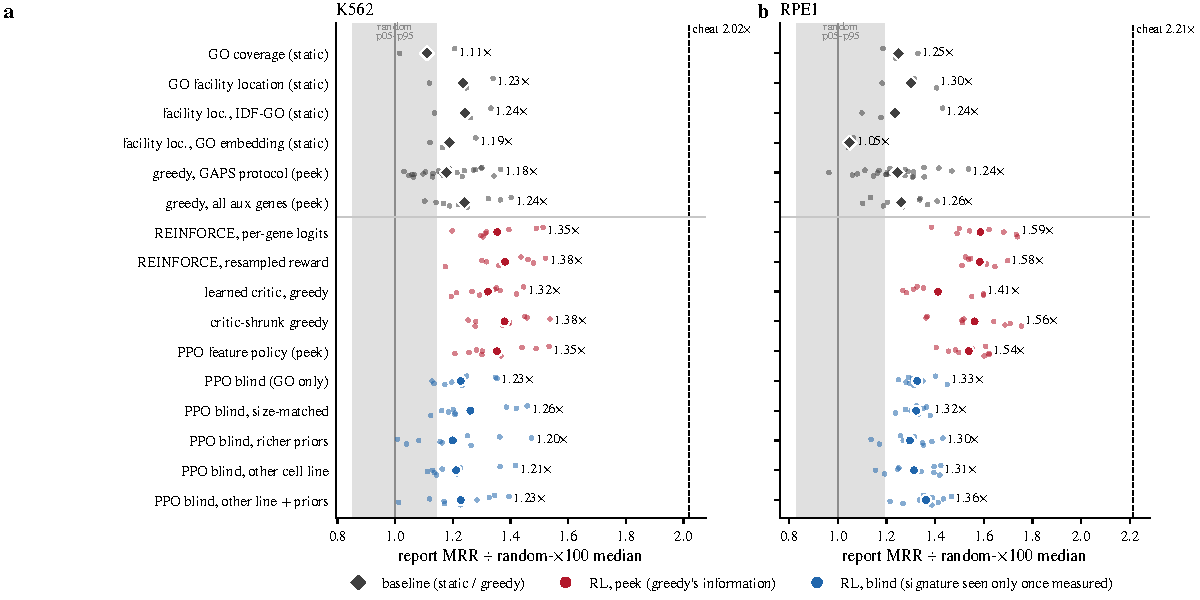
\includegraphics[width=\linewidth]{figures/fig15_rl_acquisition.pdf}
\caption{\textbf{Acquisition, budget $100$ of $437$, two Replogle screens.} Report MRR
$\div$ the split's random-$\times100$ median; small marks are split$\times$seed
($3{\times}3$), large marks the mean. Grey band = random p05--p95; dashed line = best
cheating run. \emph{Peek} RL (red) beats every baseline (grey diamonds) and clears random
p95; \emph{blind} RL (blue), where a signature is read only once measured, lands on the
static GO facility-location floor.}
\label{fig:acq}
\end{figure}

\begin{figure}[h]
\centering
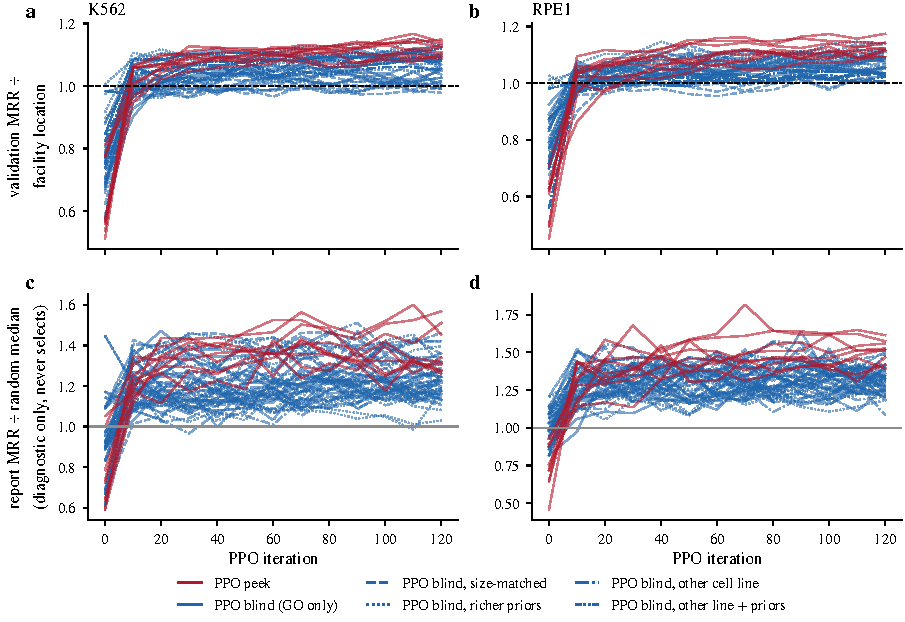
\includegraphics[width=\linewidth]{figures/fig16_rl_curves.pdf}
\caption{\textbf{PPO learning curves} (K562 left, RPE1 right). \textbf{a,b}, validation MRR
$\div$ facility location on sub-problems drawn like training ones --- every variant learns a
small ($1.03$--$1.11\times$) advantage there. \textbf{c,d}, report MRR $\div$ random median
at deployment scale (diagnostic, never used for selection): the peek policy (red) transfers;
the blind variants (blue) do not clear the facility floor. The gap between b and d is the
negative result of \Cref{sec:blind}.}
\label{fig:curves}
\end{figure}

\subsection{A clean negative result: the blind regime ties a 1970s heuristic}
\label{sec:blind}

In the blind regime --- genuine prospective design --- the PPO policy only \emph{matches}
GO facility location~\citep{nemhauser1978submodular}, a greedy set-cover on GO-Jaccard that
uses no signatures at all. We treated this as an engineering gap and named three suspects:
training sub-problems smaller than deployment, a GO-only view of a gene, and too small a
training atlas. We ran one variant each plus the combination --- $4$ variants
$\times\,2$ datasets $\times\,3$ splits $\times\,3$ seeds $=72$ runs --- and \textbf{all four
land on the static floor} ($|t|\le1.4$ paired, win rates $3/9$--$6/9$; the largest blind
number anywhere is $t{=}{+}0.54$). The scale hypothesis is \emph{refuted}, not merely
unconfirmed: size-matching the sub-problems to deployment ($437$ candidates, budget $100$)
\emph{lowered} the policy's validation advantage over facility location ($1.085\times\to
1.028\times$ on K562), so that advantage was never large enough to survive transfer --- the
earlier $5$--$13\%$ validation gain was reading noise in a small validation set. Richer
priors do not help statically either: facility location under an IDF-weighted GO view
($1.24\times$/$1.24\times$) or a $32$-dim GO-embedding view ($1.19\times$/$1.05\times$) is no
better than plain Jaccard ($1.23\times$/$1.30\times$). The honest statement of the project's
RL result is therefore a \emph{separation}: \emph{seeing the candidates' signatures is worth
$1.35$--$1.59\times$; prior knowledge alone is worth $1.23$--$1.30\times$, and a classical
heuristic already extracts all of it.} A negative result with a refuted mechanism is a
result --- it tells the next person the lever is the gene representation, not the policy.

\subsection{Published methods on the identical task}
\label{sec:related}

We ran the closest prior work through its own code on our exact splits, budget, predictor
and report genes (\Cref{fig:related}; $270$ runs, $0$ errors). \textbf{Blind:}
IterPert~\citep{huang2024iterpert} --- sequential design of Perturb-seq screens, originally
benchmarked on this same K562 screen --- and the eight active-learning methods it was
compared against (Core-Set~\citep{sener2018coreset}, BALD, BatchBALD, BADGE, LCMD, ACS-FW,
$k$-means, TypiClust) \emph{all land below} the static GO floor ($0.99$--$1.18\times$ vs
$1.23$--$1.30\times$, $t$ from $-2.1$ to $-9.3$); IterPert itself is statistically
indistinguishable from random on K562 ($1.02\times$). Our PPO-blind beats every one of them.
A $2{\times}2$ isolates why: switching the \emph{rule} from $k$-centre (IterPert's) to
facility location gains $+0.09$ to $+0.28\times$, while switching the \emph{prior} from GO to
IterPert's eight multimodal kernels (protein-language-model, text, network, imaging screens,
the other cell line) is worth essentially nothing. This closes the representation question
of \Cref{sec:blind}: those are exactly the sequence/expression/pathway priors we flagged as
untested, and they tie GO. \textbf{Peek:} data valuation (Data
Shapley~\citep{ghorbani2019datashapley}, Banzhaf~\citep{wang2023databanzhaf},
datamodels~\citep{ilyas2022datamodels}) with REINFORCE's evaluation budget beats greedy
($1.22$--$1.31\times$/$1.43$--$1.51\times$) but \emph{trails} the RL methods; a linear
(datamodels) fit explains $60\%$ of the reward's variance and the unexplained interaction
part is what optimising the set jointly buys.

\begin{figure}[h]
\centering
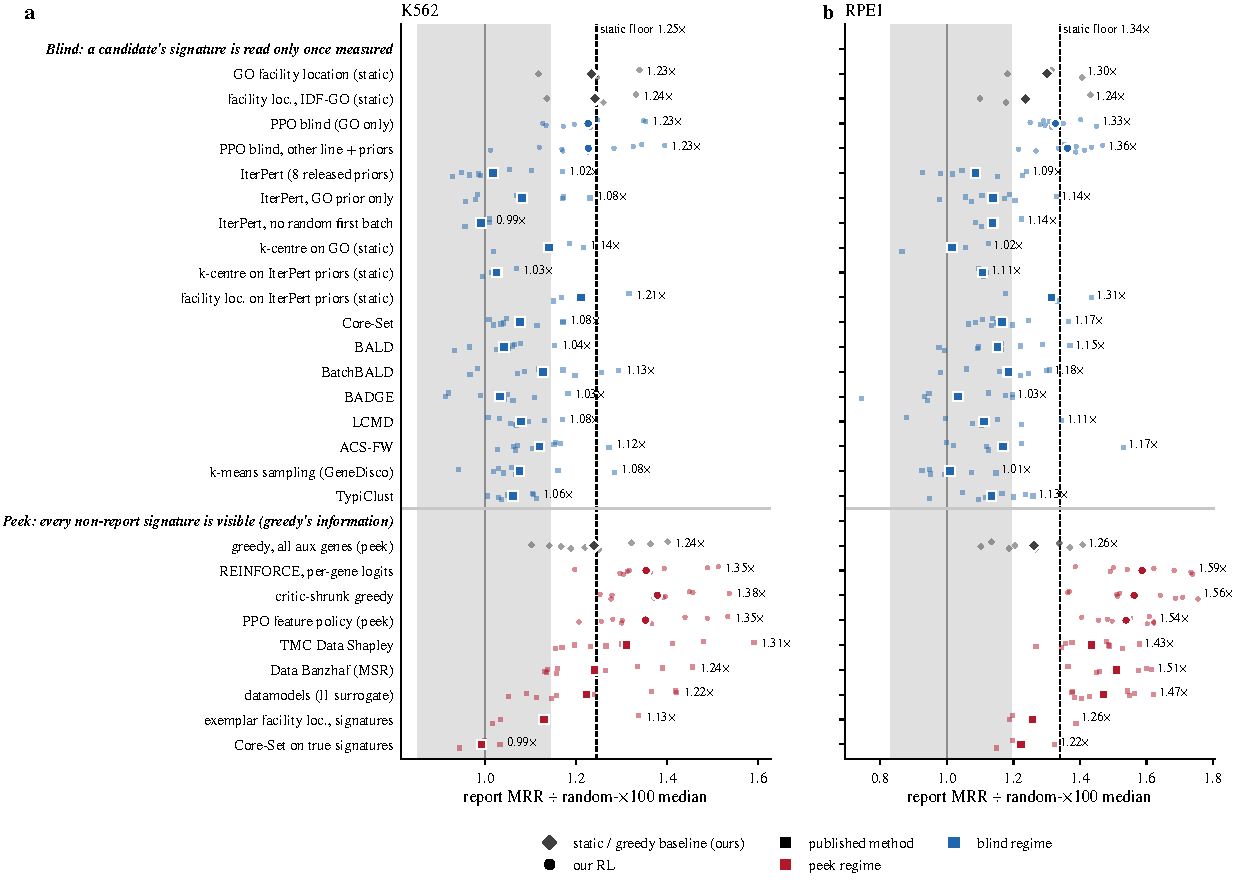
\includegraphics[width=\linewidth]{figures/fig17_related_work.pdf}
\caption{\textbf{Published acquisition methods, identical task.} Our RL (circles) and
baselines (diamonds) beside published methods (squares); red = peek regime, blue = blind.
Dashed line = our best static floor. Blind: every published method is below the floor and
below our PPO-blind. Peek: data valuation beats greedy but trails our RL.}
\label{fig:related}
\end{figure}

\subsection{Case studies: where the RL gain comes from, gene by gene}
\label{sec:cases}

Aggregates can hide a wash of wins and losses, so we follow named genes through the same
measurements (\Cref{fig:flow,fig:anatomy}). Under REINFORCE's atlas the number of report
genes identified at rank 1 rises from $4\to16$ on K562 and $0\to23$ on RPE1, with far more
genes improving $\ge2\times$ than worsening ($52$ vs $13$ of $182$; $92$ vs $24$ of $257$).
The losses are real and drawn. \Cref{fig:anatomy} dissects the largest rescue: \emph{ATP6V0C}
is never measured, so its signature is predicted from its $10$ GO-closest measured genes. A
random atlas lends it housekeeping neighbours with GO overlap $<0.18$; REINFORCE's atlas
contains \emph{ATP6V1B2}, another V-ATPase subunit (GO overlap $0.44$, signature cosine
$0.66$), lifting the prediction's cosine to truth $0.40\to0.55$ and \emph{ATP6V0C}'s rank
$\#20\to\#1$. REINFORCE chose \emph{ATP6V1B2} in all three seeds; facility location did not.
This is the deployment reward being optimised directly --- \emph{ATP6V1B2} is worth measuring
\emph{because of} report genes like \emph{ATP6V0C} --- not a generic diversity rule.
\Cref{app:extra} (\Cref{fig:gap,fig:noise}) shows the prediction crowding that makes the gap
hard, and visualises the $r{=}0.17$ reward noise directly (greedy's pick at the median
decision ranks $\#203$ of $363$ on held-out gain).

\begin{figure}[h]
\centering
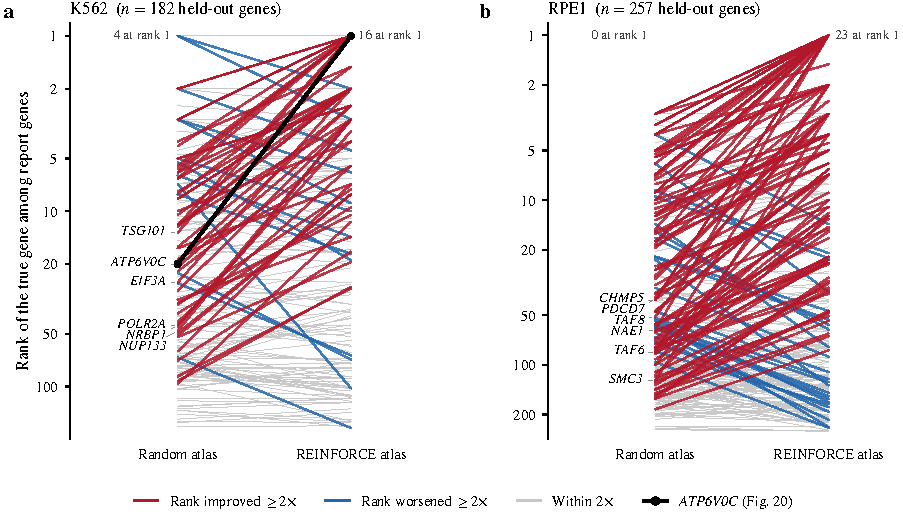
\includegraphics[width=0.88\linewidth]{figures/fig19_rescue_flow.pdf}
\caption{\textbf{Where REINFORCE's gain lands, gene by gene.} Each line joins a held-out
report gene's rank under a typical random atlas (left) to its rank under REINFORCE's atlas
(right). Red: improved $\ge2\times$; blue: worsened $\ge2\times$; black: \emph{ATP6V0C}
(\Cref{fig:anatomy}). \textbf{a}, K562 ($n{=}182$). \textbf{b}, RPE1 ($n{=}257$).}
\label{fig:flow}
\end{figure}

\begin{figure}[h]
\centering
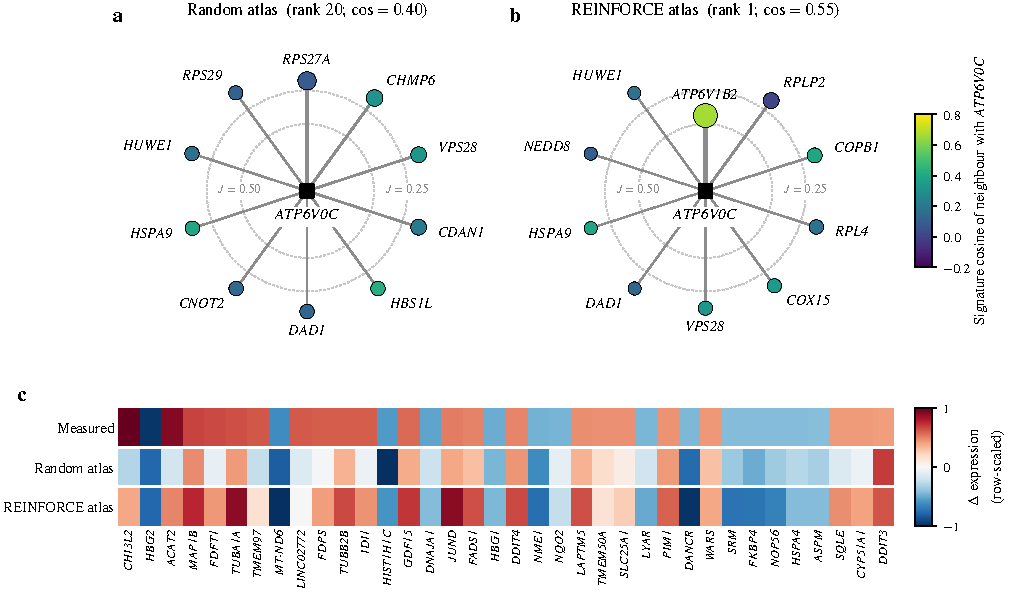
\includegraphics[width=\linewidth]{figures/fig20_rescue_anatomy.pdf}
\caption{\textbf{One rescue dissected: \emph{ATP6V0C} (K562).} \textbf{a,b}, its $10$ GO-kNN
neighbours in a random atlas vs REINFORCE's; radial distance $=1-$ GO Jaccard, marker
size/spoke width $\propto$ kNN weight, colour $=$ signature cosine with \emph{ATP6V0C}.
Measuring the V-ATPase subunit \emph{ATP6V1B2} (lower-left in b) moves the rank $\#20\to\#1$.
\textbf{c}, its $36$ most-changed readout genes: measured, and predicted from each atlas.}
\label{fig:anatomy}
\end{figure}

\begin{AIbox}{Takeaways}
\footnotesize
\textbf{(1) Measure the reward before post-training the generator.} Ceiling $86.6\%$ vs
GEARS $8.3\%$: the oracle, not the generator, caps this task, so distribution-matching
post-training has no visible headroom. \textbf{(2) The RL-shaped problem is acquisition.}
Choosing $100$ of $437$ genes is a combinatorial MDP with a discrete action space and a
high-variance reward ($r{=}0.17$ to the quantity that matters). \textbf{(3) With greedy's
information, RL wins.} REINFORCE / critic-control-variate / PPO-GRPO reach
$1.35$--$1.59\times$ random and beat greedy in $85/90$ paired runs; each isolates one cause
(search / reward estimate / generalisation). \textbf{(4) The negative result is sharp.} In
the prospective (blind) regime five learned policies tie a 1970s facility-location
heuristic, and the scale hypothesis is \emph{refuted}; the binding constraint is the gene
representation, confirmed by IterPert's eight multimodal priors tying GO.
\end{AIbox}

\section{Datasets, Environments, and Resources [2 points]}

\textbf{Data.} GEARS-processed Perturb-seq: Replogle K562 \& RPE1
essential~\citep{replogle2022perturbseq} ($\sim$163k cells, $1{,}092$/$1{,}543$ perturbed
conditions --- the two action spaces large enough to be real), plus
Norman~\citep{norman2019gi}, Adamson~\citep{adamson2016upr} and
Dixit~\citep{dixit2016perturbseq} for the feasibility probes and the GO
graph. All derived state is written to disk (JSONL rows, \texttt{npz} profiles) so every
figure is redrawable without recomputation. \textbf{The acquisition MDP is an offline
simulator}: episodes are matrix operations over cached real signatures (a $57$--$69$\,MB
\texttt{npz} per dataset), with \emph{no} GEARS forward pass in the loop --- the one place
we deliberately avoid the oracle, since \Cref{sec:oracle} shows it would only inject noise.
\textbf{Environments.} Two pinned envs (an analysis env: scanpy 1.12 / numpy 2.4 /
matplotlib 3.11; a torch env: torch 2.4.1+cu121 / PyG 2.6.1 / numpy${<}2$, the last required
because GEARS' own pickles reference a numpy path removed in 2.x). \textbf{Compute.} All work
runs through SLURM as CPU jobs --- profiling, the oracle probe, the baselines/training
arrays, the figures. The RL runs need \emph{no GPU} (they are offline matrix ops), which is
itself a practical finding: the headline RL study is $\sim$$10$--$30$ CPU-core-hours, not GPU
time. Figures are generated by CPU viz jobs that read saved artifacts only; every job prints
its host, resource request and gates so a partial result cannot masquerade as success.

\section{Updated Plan and Next Steps [5 points]}

\textbf{What is done.} Milestone 1 (baselines, data, oracle weights, environments) is
complete; we are ahead on analysis and already have the core RL results and an honest
related-work table. The pivot above \emph{is} the ``extend the framework to problems
encountered'' step in the proposed timeline, done early and with measurements behind it.

\textbf{Remaining work (now $\to$ Dec 7).}
\begin{enumerate}[leftmargin=1.4em,itemsep=1pt,topsep=2pt]
  \item \textbf{(Now--Nov 25) Attack the one open problem the negative result isolates:} a
  \emph{prospective} policy needs a gene representation that predicts \emph{effect}, not GO
  category. GO, IDF-GO, GO-embedding and IterPert's eight multimodal priors all tie; we will
  test sequence (ESM), expression co-variation and pathway-topology features \emph{inside the
  predictor} (gap 0's question), not only inside the policy, and re-run the blind table. A
  blind policy can only beat facility location if its features see effect.
  \item \textbf{(Now--Nov 25) Strengthen the RL story we already have:} ablate the critic
  control-variate weight $\lambda$ and the GRPO group size; add seeds to tighten the
  $n{=}9$ estimates; report learning-curve variance. The critic-as-control-variate result
  (diagnostic $r{:}0.17\to0.26$, $18/18$ wins) is the cleanest RL contribution and deserves
  a focused ablation.
  \item \textbf{(Nov 25--Dec 1) Close the loop back to the oracle:} retrain GEARS held-out
  (\texttt{split=simulation}) to confirm the oracle rung on data it has \emph{not} seen; if
  the held-out margin over the non-conditional baseline is thin, swap in STATE~\citep{arcstate2026}
  (already cloned) and re-measure the ladder.
  \item \textbf{(Dec 1--7) Final experiments + writeup:} consolidate tables, finalise the
  peek/blind separation as the headline, and the case studies as the mechanism.
\end{enumerate}

\textbf{Risks and mitigations.} \emph{(i) The open problem may stay negative} --- richer
representations might also tie facility location. Mitigation: a tie is still a publishable,
well-measured separation, and we have it already; the upside case is a representation that
breaks it. \emph{(ii) Small $n$ per setting.} Mitigation: every number is already expressed
against its split's random distribution with p95/max, and greedy/cheat are run over seeds
because a single draw spans $\pm15\%$. \emph{(iii) Scope creep back toward generation.}
Mitigation: the acquisition MDP is the committed deliverable; a generator comparison
(RL policy vs LabCompass~\citep{labcompass2026} guidance on a non-differentiable reward)
is a stretch goal, not a dependency.

\section{Team Contributions}

Both members are CMU students; the workload re-balanced around the pivot from generation to
acquisition. \textbf{Yixi Zhao} --- forward/inverse oracle probing and the ceiling/oracle
ladder (\Cref{sec:oracle}), the generalization-axis study (\Cref{fig:headroom}), the
acquisition MDP simulator, REINFORCE (Plackett--Luce) and the learned critic / control-variate,
and the static baselines (facility location, multi-seed greedy, the cheating bound).
\textbf{Zhangchi (Allen) Chen} --- the PPO/GRPO feature policy, the blind-regime variants
(size-matched / cross-line / richer-prior) and the learning-curve and gradient-attribution
diagnostics, the related-work harness (IterPert + bmdal AL methods + data valuation through
their own code), and the case-study figures. The GEARS environment, evaluation fixes
(duplicate conditions, Ensembl-vs-name), writing, and the SLURM job/figure pipeline were
shared.

\section{Reflection and Feedback}

\textbf{What we learned.} The most useful RL lesson was not an algorithm but a discipline:
\emph{measure the reward, and the baseline, before optimising.} The project would have spent
weeks post-training a generator against a reward (GEARS) that cannot discriminate, and would
have ``beaten random'' at acquisition without noticing that a 1970s heuristic and the random
distribution's own $\pm15\%$ spread were the real bars. Concretely we learned why variance
reduction matters \emph{here} (a reward that correlates $r{=}0.17$ with its target actively
harms greedy), how a one-step critic doubles as a reward-quality diagnostic, and that a
GRPO-style group baseline is a natural fit for an episodic set-reward with no per-step signal.
We also learned to value a negative result: refuting our own scale hypothesis (the validation
advantage was never there) was more informative than any incremental positive.

\textbf{Feedback we would like.} (1) Is a well-measured \emph{separation} plus a
mechanism-backed negative result an acceptable core contribution for the final report, or
should we weight the stretch generator-vs-guidance comparison more? (2) Pointers on gene
representations that encode \emph{effect} rather than annotation --- this is the one input
that could flip the blind regime. (3) A sanity check on our offline-MDP evaluation protocol
(three-way \texttt{act}/\texttt{rew}/\texttt{rep} splits, scoring against the random-$\times$100
distribution): is there a standard we should match? Compute has not been a blocker --- the RL
is CPU-only --- so our ask is methodological rather than resource.

\bibliography{main,refs}

\newpage
\appendix
\onecolumn
\part*{Appendices}

\section{Additional case studies}
\label{app:extra}

\begin{figure}[h]
\centering
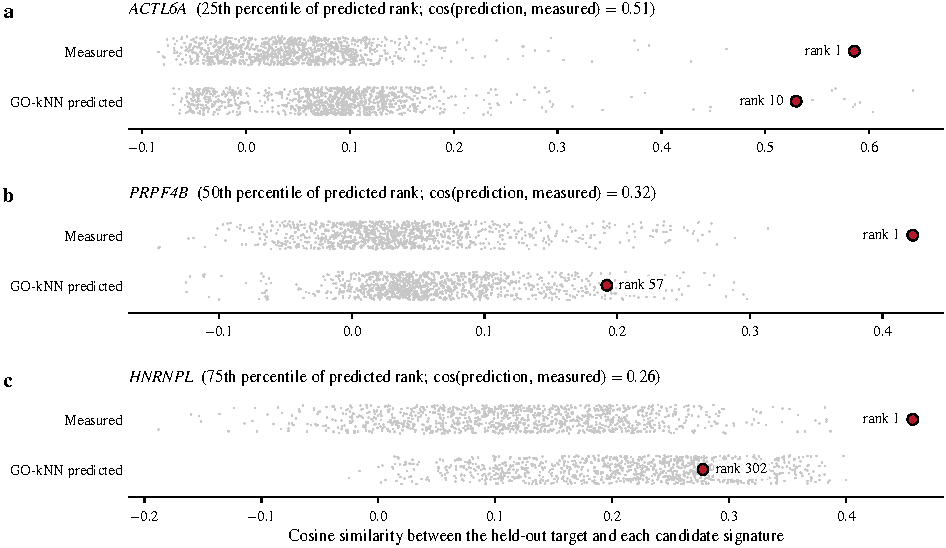
\includegraphics[width=0.95\linewidth]{figures/fig18_gap_crowd.pdf}
\caption{\textbf{The unseen-gene gap, one gene at a time (K562).} A held-out target scored
against all candidates by their measured signatures (top of each panel) and their GO-kNN
predictions (bottom); red dot = the true gene, with its rank. \textbf{a--c}, the genes at
the $25$th/$50$th/$75$th percentile of predicted rank among the $371$ the measurement ranks
first. Predictions are not wrong in direction (cosine $0.26$--$0.51$); they \emph{crowd},
so the target cannot pick its own out --- discrimination, not fidelity.}
\label{fig:gap}
\end{figure}

\begin{figure}[h]
\centering
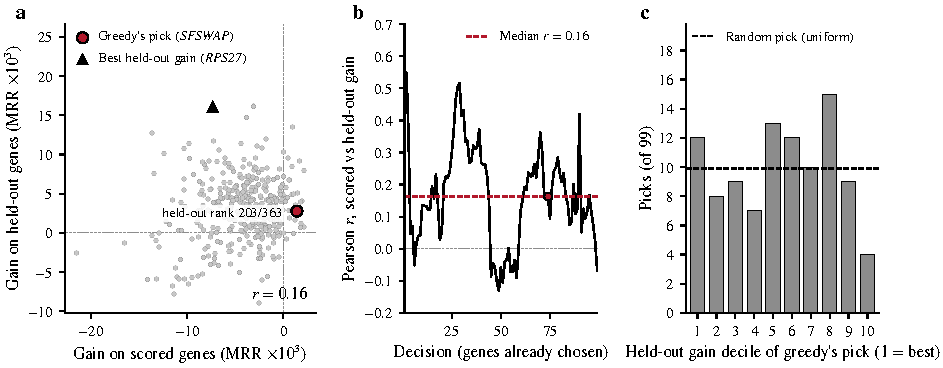
\includegraphics[width=\linewidth]{figures/fig21_greedy_noise.pdf}
\caption{\textbf{Greedy's scored gain barely predicts held-out gain (K562)} --- the reward
noise of \Cref{sec:mdp,sec:methods} visualised. \textbf{a}, at the median decision, each
candidate's gain on the genes greedy is scored on vs its gain on held-out genes
($r{=}0.16$); greedy's pick \emph{SFSWAP} ranks $\#203/363$ held-out. \textbf{b}, that
correlation at each of greedy's $99$ decisions. \textbf{c}, where greedy's picks landed by
held-out gain, in deciles --- only $12$ of $99$ reach the top decile, against $\sim\!10$ for
random. Greedy's atlas still helps overall (almost any gene helps); what it cannot do is
tell the better candidates from the rest, which is what the RL methods add.}
\label{fig:noise}
\end{figure}

\end{document}
